\documentclass[pdflatex,compress]{beamer}

%\usetheme[dark,framenumber,totalframenumber]{ElektroITK}
\usetheme[darktitle,framenumber,totalframenumber]{ElektroITK}

\usepackage{graphicx}
\usepackage{multicol}

\title{METODE NUMERIK}
\subtitle{Solusi Persamaan Nirlanjar}

\author{Tim Dosen Pengampu}

\begin{document}
	
\maketitle

\begin{frame}
	\frametitle{Rumusan Masalah}
	\begin{itemize}
		\item \textbf{Persoalan:} Temukan nilai $ x $ yang memenuhi persamaan
		\[f(x) = 0\]
		yaitu nilai $ x = s $ sedemikian sehingga $ f(s) = 0 $.
		\item Nilai $ x = s $ disebut \textbf{akar} persamaan $ f(x) = 0 $
	\end{itemize}
\end{frame}

\begin{frame}
	\frametitle{Contoh persoalan dalam bidang elektronika}
	Suatu arus osilasi dalam rangkaian listrik diberikan oleh
	
	\[ I = 10e^{-t}\sin(2 \pi t) \]
	
	yang dalam hal ini $ t $ dalam detik. Tentukan semua nilai $ t $
	sedemikan sehingga $ I = 2 $ ampere.\\
	Persoalan ini adalah mencari nilai $ t $ sedemikian sehingga:

	\[ 10e^{-t} \sin(2 \pi t) – 2 = 0 \]
\end{frame}

\begin{frame}
	\frametitle{Metode Pencarian Akar}
	\begin{enumerate}
		\item Metode tertutup (bracketing method)
		\begin{itemize}
			\item Mencari akar di dalam selang $ [a, b] $.
			\item Selang $ [a, b] $ sudah dipastikan berisi minimal satu buah akar.
			\item Karena itu metode jenis ini selalu berhasil menemukan akar.
			\item Dengan kata lain, lelarannya selalu konvergen (menuju) ke akar,
			\item Karena itu metode tertutup kadang-kadang dinamakan juga \textbf{metode konvergen}.
		\end{itemize}
	\end{enumerate}
\end{frame}

\begin{frame}
	\begin{enumerate}
		\setcounter{enumi}{1}
		\item Metode terbuka
		\begin{itemize}
			\item Tidak memerlukan selang $ [a, b] $ yang mengandung akar.
			\item Mencari akar melalui suatu lelaran yang dimulai
			dari sebuah tebakan (\textit{guest}) awal.
			\item Pada setiap lelaran kita menghitung hampiran akar yang baru.
			\item Mungkin saja hampiran akar yang baru mendekati akar sejati (konvergen), atau mungkin juga menjauhinya (divergen).
			\item Karena itu, metode terbuka tidak selalu berhasil menemukan akar, kadang-kadang konvergen, kadangkala ia divergen.
		\end{itemize}
	\end{enumerate}
\end{frame}

\begin{frame}
	\frametitle{Metode Tertutup}
	\begin{itemize}
		\item Diperlukan selang $ [a, b] $ yang mengandung minimal satu buah akar.
		\item Syarat cukup keberadaan akar: Jika $ f(a) f(b) < 0 $ dan $ f(x) $ menerus di dalam selang $ [a, b] $, maka paling sedikit terdapat satu buah akar persamaan f(x) = 0 di dalam selang $ [a, b] $.
		\item Dengan kata lain: selang $ [a, b] $ harus berbeda tanda pada nilai-nilai fungsinya supaya terdapat minimal 1 buah akar.
	\end{itemize}
\end{frame}

\begin{frame}
	\frametitle{Syarat cukup keberadaan akar}
	\begin{center}
		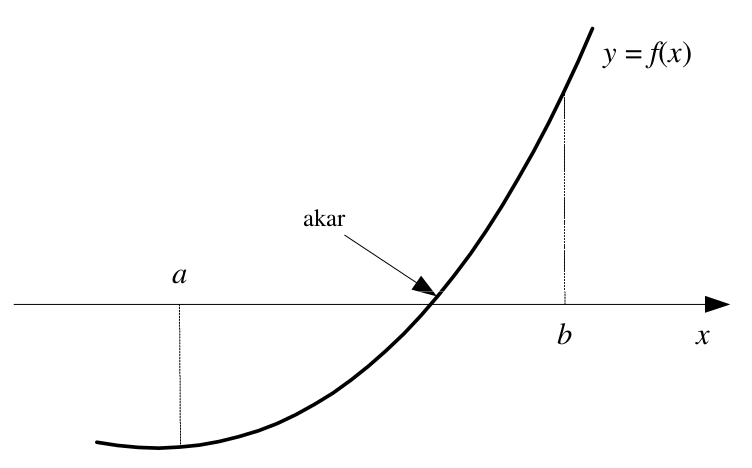
\includegraphics[width=1\linewidth]{img/img01}
	\end{center}
\end{frame}

\begin{frame}
	\frametitle{Kondisi yang mungkin terjadi}
	\begin{enumerate}
		\item $ f(a)f(b) < 0 $, maka terdapat akar sebanyak bilangan ganjil.
		\begin{center}
			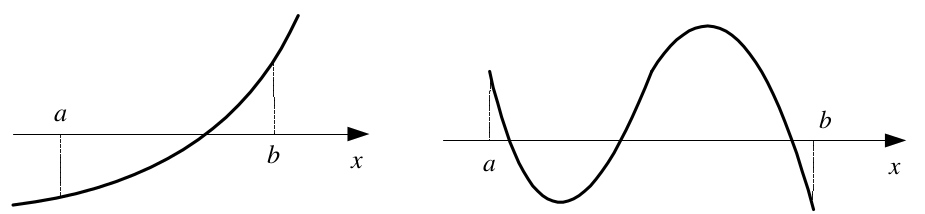
\includegraphics[width=0.8\linewidth]{img/img02}
		\end{center}
		\item $ f(a)f(b) > 0 $, maka terdapat akar sebanyak bilangan genap (termasuk tidak ada akar).
		\begin{center}
			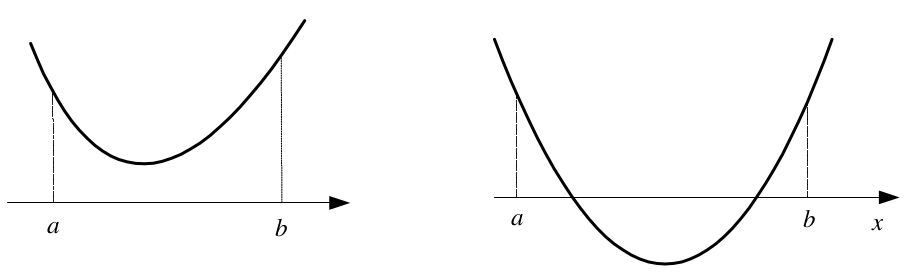
\includegraphics[width=0.8\linewidth]{img/img03}
		\end{center}
	\end{enumerate}
\end{frame}

\begin{frame}
	\begin{itemize}
		\item Cara menentukan selang yang cukup kecil dan mengandung akar:
		\begin{enumerate}
			\item Membuat grafik fungsi di bidang X-Y, lalu melihat di mana perpotongannya dengan sumbu-X.
			\item Membuat tabel yang memuat nilai-nilai fungsi pada pada titik-titik absis yang berjarak tetap (h).Nilai h dibuat cukup kecil. (lihat contoh berikut)
		\end{enumerate}
	\end{itemize}
\end{frame}

\begin{frame}
	\begin{itemize}
		\item \textbf{Contoh:} Tabel nilai-nilai $ f(x) = e^x - 5x^2 $ mulai dari $ a = -0.5 $ sampai $ b = 1.4 $ dengan kenaikan absis sebesar $ h = 0.1 $		
	\end{itemize}
	\begin{multicols}{2}
	\begin{center}
		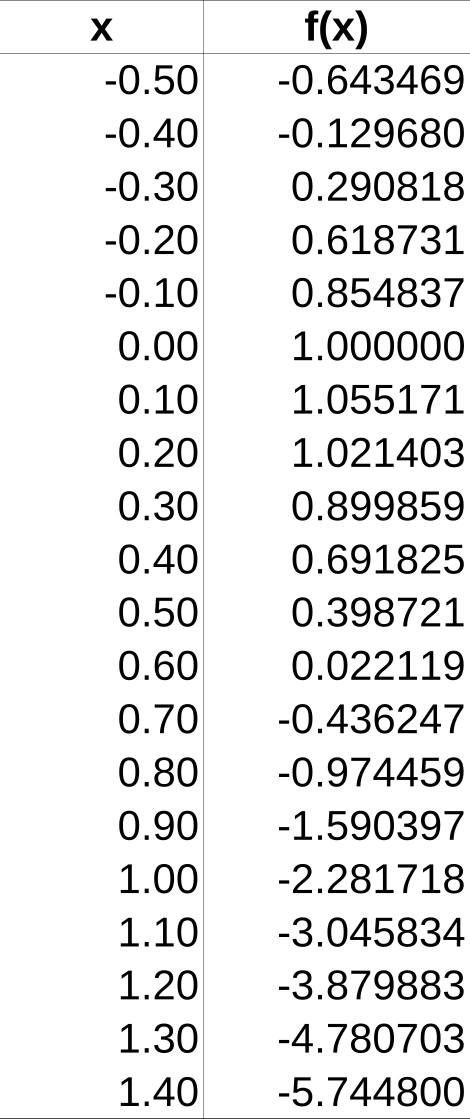
\includegraphics[width=0.5\linewidth]{img/img04.png}
	\end{center}
	\columnbreak
	Selang-selang yang dapat dipilih dan mengandung akar:
	\begin{enumerate}
		\item $ [-0.40, -0.30] $
		\item $ [0.60, 0.70] $
		\item $ [0.50, 0.70] \rightarrow $ Bisa dipilih, tetapi cukup lebar.
		\item $ [-0.50, -0.20] \rightarrow $ Bisa dipilih, tetapi cukup lebar.
	\end{enumerate}			
	\end{multicols}
\end{frame}

\begin{frame}
	\begin{itemize}
		\item Metode Tertutup ada dua:
		\begin{enumerate}
			\item Metode bagidua
			\item Metode regula-falsi
		\end{enumerate}
	\end{itemize}
\end{frame}

\begin{frame}
	\frametitle{Metode Bagidua (Bisection Method)}
	\begin{center}
		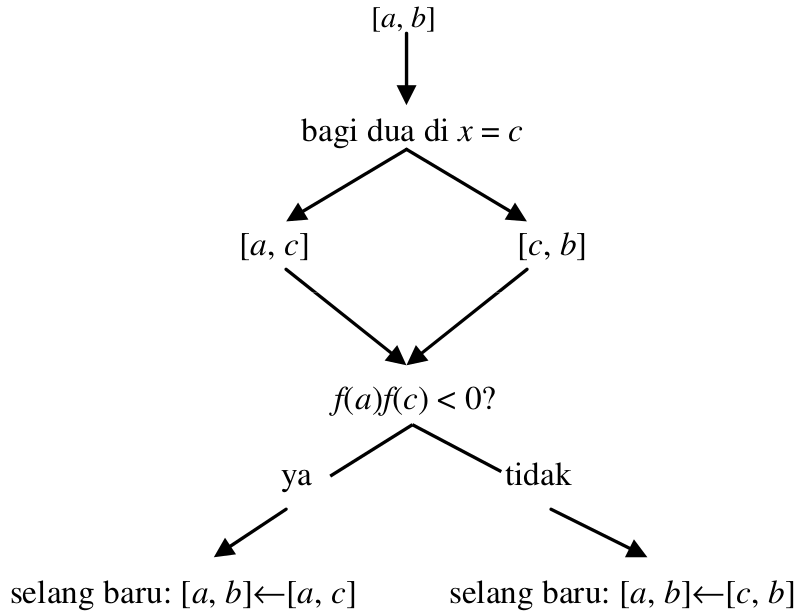
\includegraphics[width=0.7\linewidth]{img/img05.png}
	\end{center}
\end{frame}
\end{document}
